\section{User Controlled Walking}
\label{sec::51_uc}
As the fundamental building block for the comparison to autonomous walking, we now need to investigate on user controlled walking. This enables us, in contrast to the control by a neural network, to find the best parameters for the pattern generation in a well controllable environment. These parameters will then be kept constant throughout the rest of this thesis, in order to allow for a good comparison between user controlled walking and autonomously controlled walking. Furthermore, we will rely on them to gather data for the behavioral cloning approach in section \ref{sec::523_da}.
\subsection{Benchmarking of Implementation}
To evaluate the pattern generator implementation of ours, we have benchmarked it against an existing one, which was written in Python. Therefore, we defined velocity commands, as they typically may appear in real world scenarios. The four defined use cases, which are shown in figures \ref{fig::511_benchmarking_traj} and \ref{fig::511_benchmarking_advanced}, were parametrized in accordance to the HRP-2 humanoid robot.
\begin{figure}[h]
	\centering
	\subcaptionbox{Straight trajectories at\\$\bm{v}=\begin{pmatrix}
		0.1 & 0.0 & 0.0
		\end{pmatrix}^T$.}%
	[.4\linewidth]{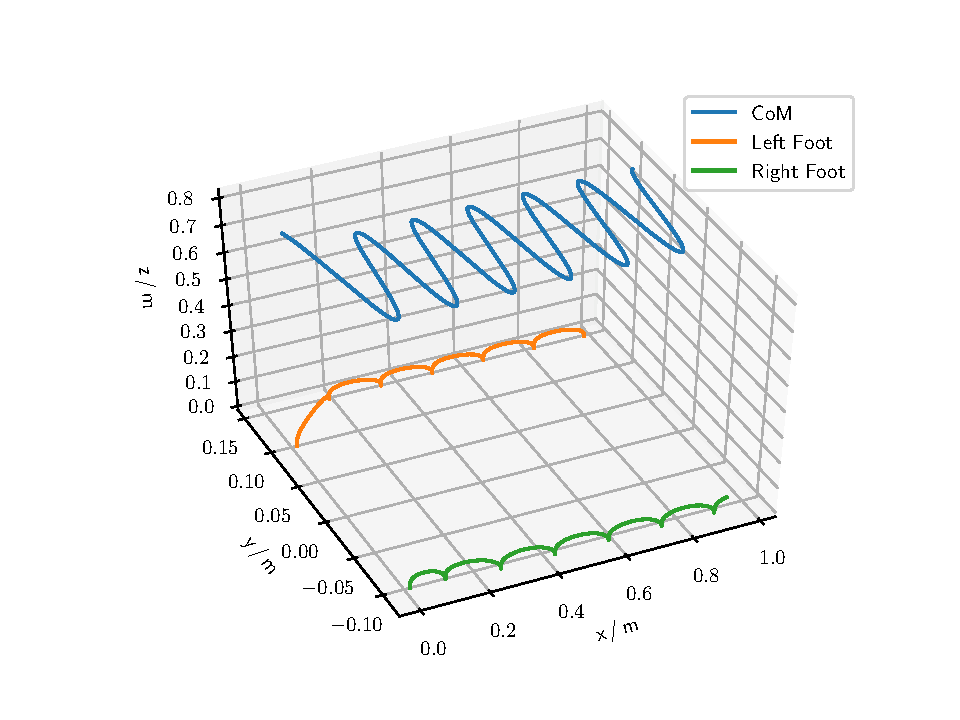
\includegraphics[scale=.35]{chapters/05_experiments/01_user_controlled_walking/01_benchmarking/nmpc_straight.pdf}}
	\subcaptionbox{Diagonal trajectories at\\$\bm{v}=\begin{pmatrix}
		0.1 & 0.1 & 0.0
		\end{pmatrix}^T$.}%
	[.4\linewidth]{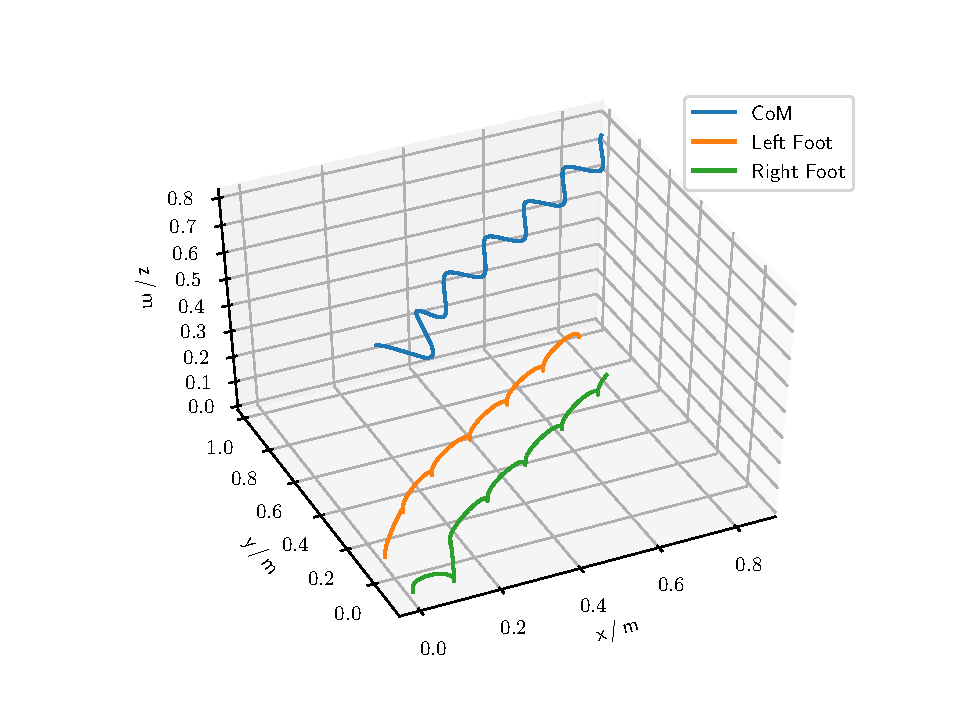
\includegraphics[scale=.35]{chapters/05_experiments/01_user_controlled_walking/01_benchmarking/nmpc_diagonal.pdf}}
	\caption{Simple trajectories. The velocities are given in units of\\$(\text{m}/\text{s}\,\,\,\,\text{m}/\text{s}\,\,\,\,\text{rad}/\text{s})^T$.}
	\label{fig::511_benchmarking_basic}
\end{figure} 
The parameters for these tests can be found in the YAML file at the provided \href{https://github.com/mhubii/nmpc_pattern_generator/blob/719fde0bb73925923de85cbf379c5523e075dfeb/libs/pattern_generator/configs_hrp2.yaml#L1}{link}. To obtain the pattern generator's performance, in terms of speed, the straight walk experiment in figure \ref{fig::511_benchmarking_basic} (a) got executed ten times on an Intel Core i7-7700HQ CPU at $2.8\,\text{GHz}$, for both, the Python and our implementation. It took $873\pm23\,\text{ms}$ and $147.7\pm0.5\,\text{ms}$ to execute the code for $100$ iterations on average, which means that a single iteration took $8.73\pm0.23\,\text{ms}$ and $1.48\pm0.01\,\text{ms}$. We therefore could achieve a speedup of around $600$ percent with our implementation. We further demonstrate the avoidance of convex obstacle with a security margin that keeps the robot at a safe distance in figure \ref{fig::511_benchmarking_advanced} (b). The used obstacle is defined to be located at $x=1.6\,\text{m}$ and $y=1.0\,\text{m}$, with a radius of $R=1.0\,\text{m}$, and a security margin of $m=0.4\,\text{m}$.
\begin{figure}[h]
	\centering
	\subcaptionbox{Curved trajectories at\\$\bm{v}=\begin{pmatrix}
	0.1 & 0.0 & 0.1
	\end{pmatrix}^T$.}%
	[.4\linewidth]{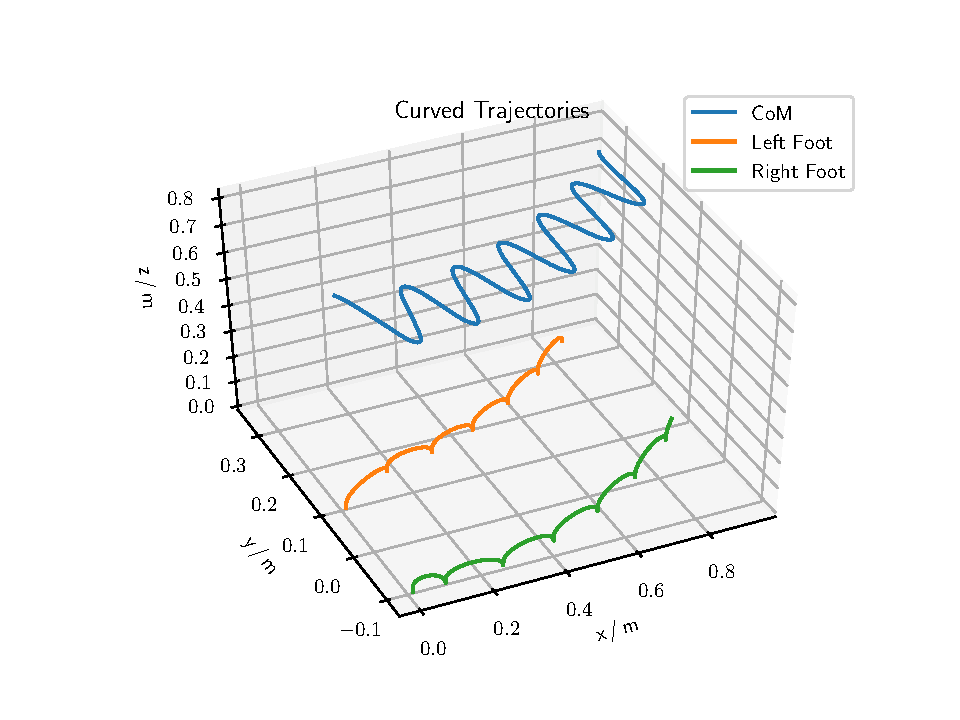
\includegraphics[scale=.35]{chapters/05_experiments/01_user_controlled_walking/01_benchmarking/nmpc_turn.pdf}}
	\subcaptionbox{Obstacle avoidance at\\$\bm{v}=\begin{pmatrix}
	0.1 & 0.0 & 0.0
	\end{pmatrix}^T$}%
	[.4\linewidth]{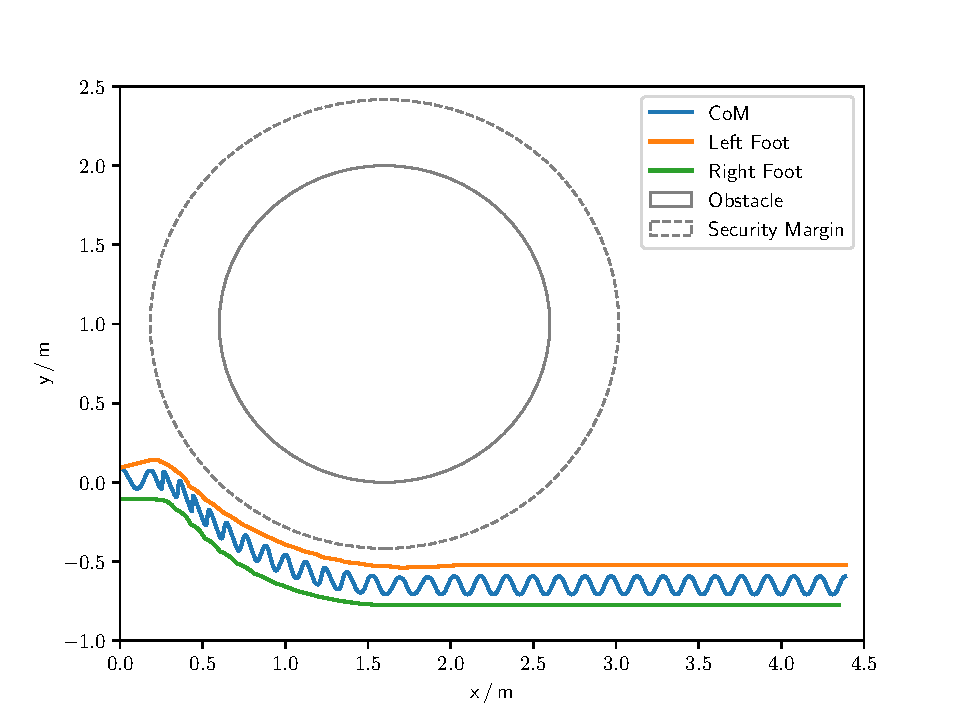
\includegraphics[scale=.35]{chapters/05_experiments/01_user_controlled_walking/01_benchmarking/nmpc_obstacle.pdf}}
	\caption{Advanced trajectories. The velocities are given in units of\\$(\text{m}/\text{s}\,\,\,\,\text{m}/\text{s}\,\,\,\,\text{rad}/\text{s})^T$.}
	\label{fig::511_benchmarking_advanced}
\end{figure} 
To ensure a smooth motion at all times, and to benchmark the interpolation, we plotted the x-, y-, and z-trajectories for the left and the right foot, as shown in figure \ref{fig::511_benchmarking_inter}. The plots were generated on the curved trajectory of figure \ref{fig::511_benchmarking_advanced} (a), and they reveal a continuous behavior at all times and for all dimensions.
\begin{figure}[h]
	\centering
	\subcaptionbox{Interpolated\\x-Trajectories}%
	[.3\linewidth]{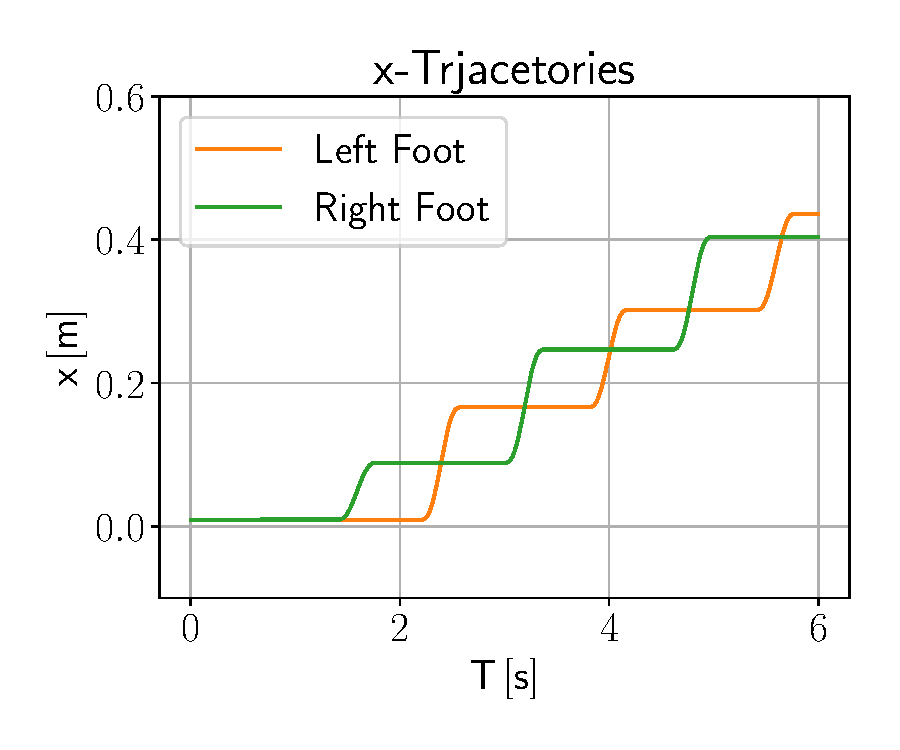
\includegraphics[scale=.3]{chapters/05_experiments/01_user_controlled_walking/01_benchmarking/interpolated_x_trajectories.pdf}}
	\subcaptionbox{Interpolated\\y-Trajectories}%
	[.3\linewidth]{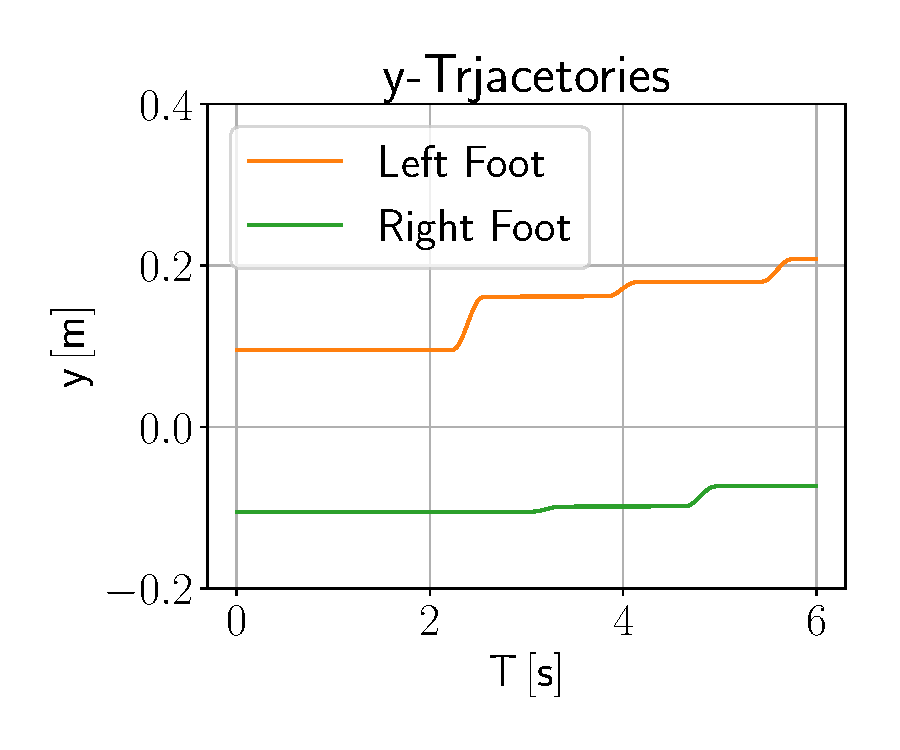
\includegraphics[scale=.3]{chapters/05_experiments/01_user_controlled_walking/01_benchmarking/interpolated_y_trajectories.pdf}}
	\subcaptionbox{Interpolated\\z-Trajectories}%
	[.3\linewidth]{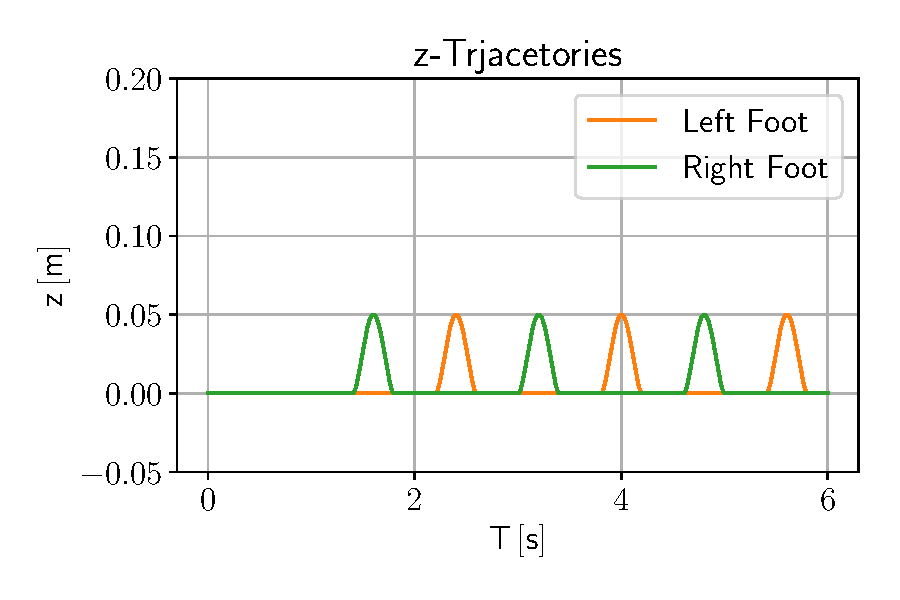
\includegraphics[scale=.3]{chapters/05_experiments/01_user_controlled_walking/01_benchmarking/interpolated_z_trajectories.pdf}}
	\caption{Interpolated foot trajectories.}
	\label{fig::511_benchmarking_inter}
\end{figure}
 The benchmarked pattern generator then enabled us to run it on the real robot, which we did in a test environment that will be presented in the next section - Performance in Test Environment.
\subsection{Performance in Test Environment}
\begin{figure}[h]
	\centering
	\subcaptionbox{Straight Walk - Dynamic Balance}%
	[.4\linewidth]{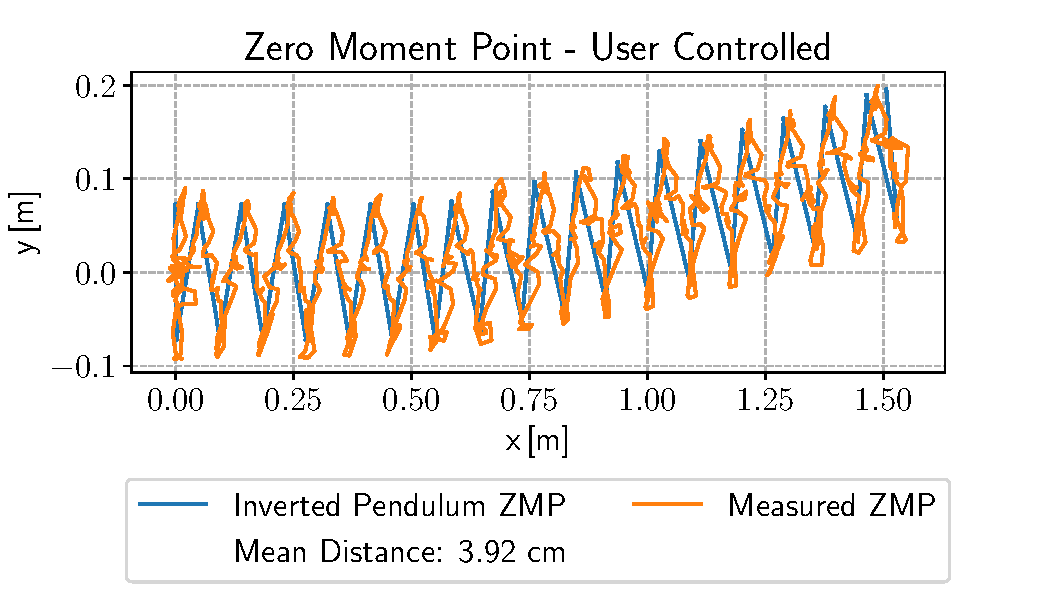
\includegraphics[scale=.35]{chapters/05_experiments/01_user_controlled_walking/02_test_environment/straight_walk_01_zmp.pdf}}
	\subcaptionbox{Straight Walk - Behavior}%
	[.4\linewidth]{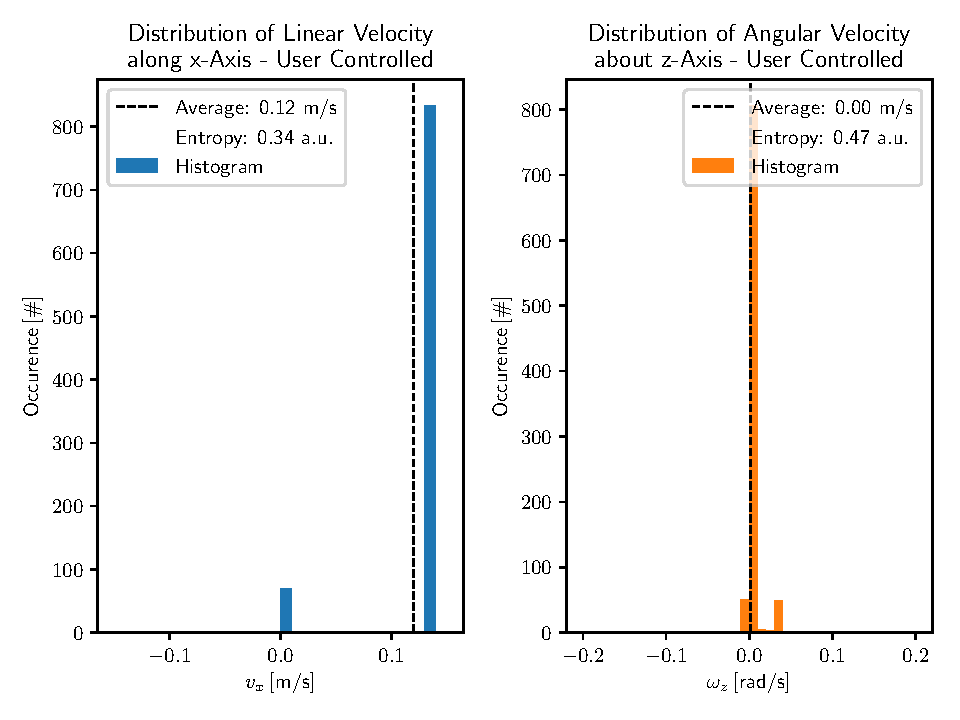
\includegraphics[scale=.35]{chapters/05_experiments/01_user_controlled_walking/02_test_environment/straight_walk_01_entropy.pdf}}
	\subcaptionbox{Curved Walk - Dynamic Balance}%
	[.4\linewidth]{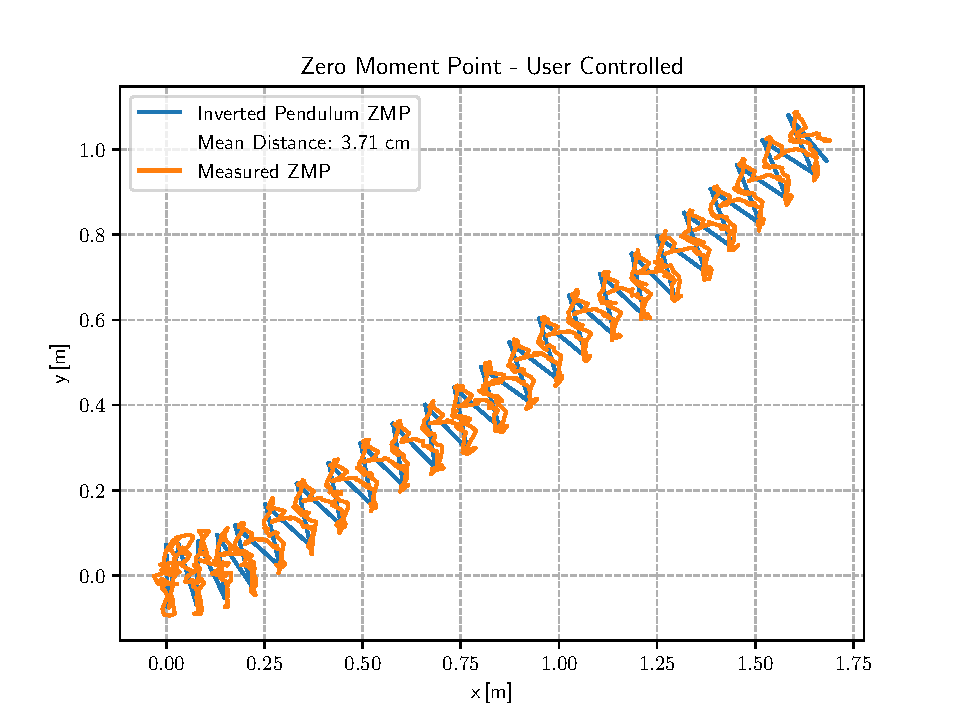
\includegraphics[scale=.35]{chapters/05_experiments/01_user_controlled_walking/02_test_environment/curved_walk_01_zmp.pdf}}
	\subcaptionbox{Curved Walk - Behavior}%
	[.4\linewidth]{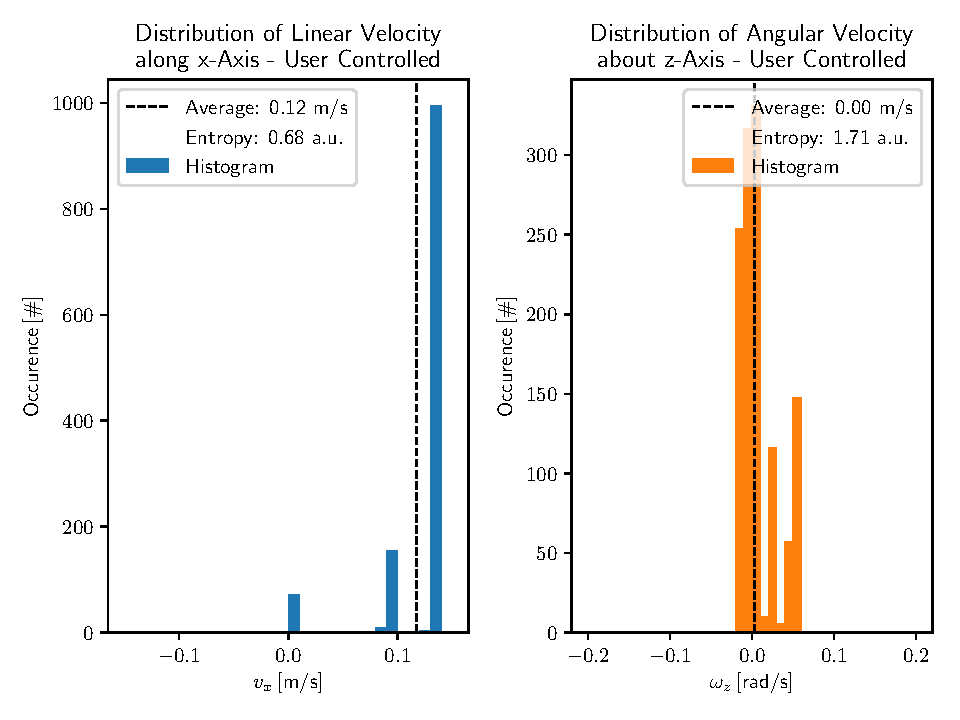
\includegraphics[scale=.35]{chapters/05_experiments/01_user_controlled_walking/02_test_environment/curved_walk_01_entropy.pdf}}
	\subcaptionbox{Obstacle Avoidance - Dynamic Balance}%
	[.4\linewidth]{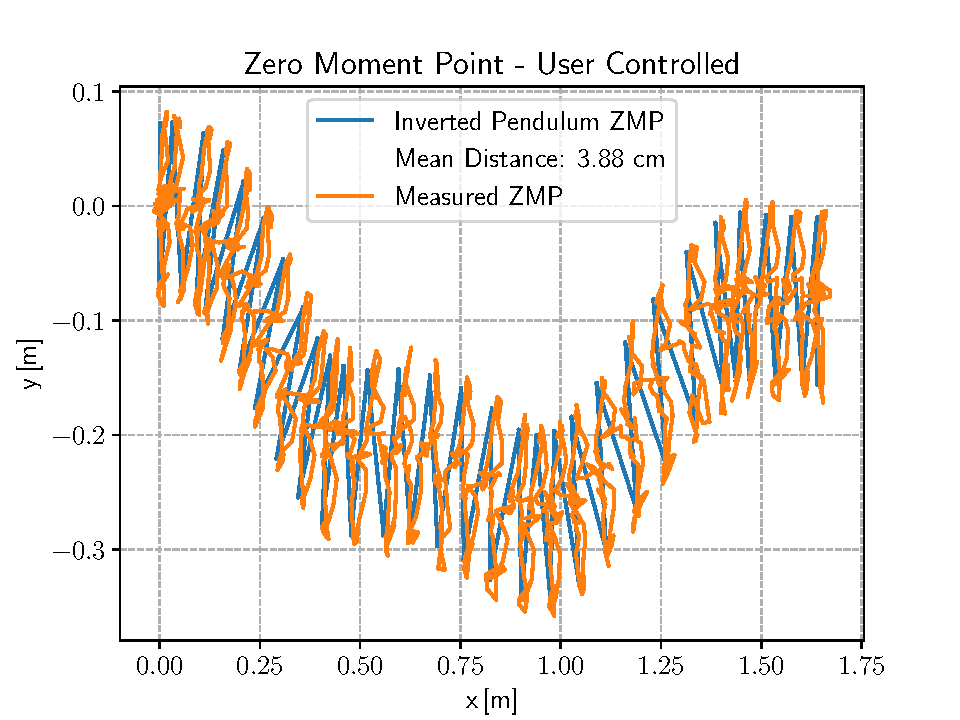
\includegraphics[scale=.35]{chapters/05_experiments/01_user_controlled_walking/02_test_environment/obstacle_walk_02_zmp.pdf}}
	\subcaptionbox{Obstacle Avoidance - Behavior}%
	[.4\linewidth]{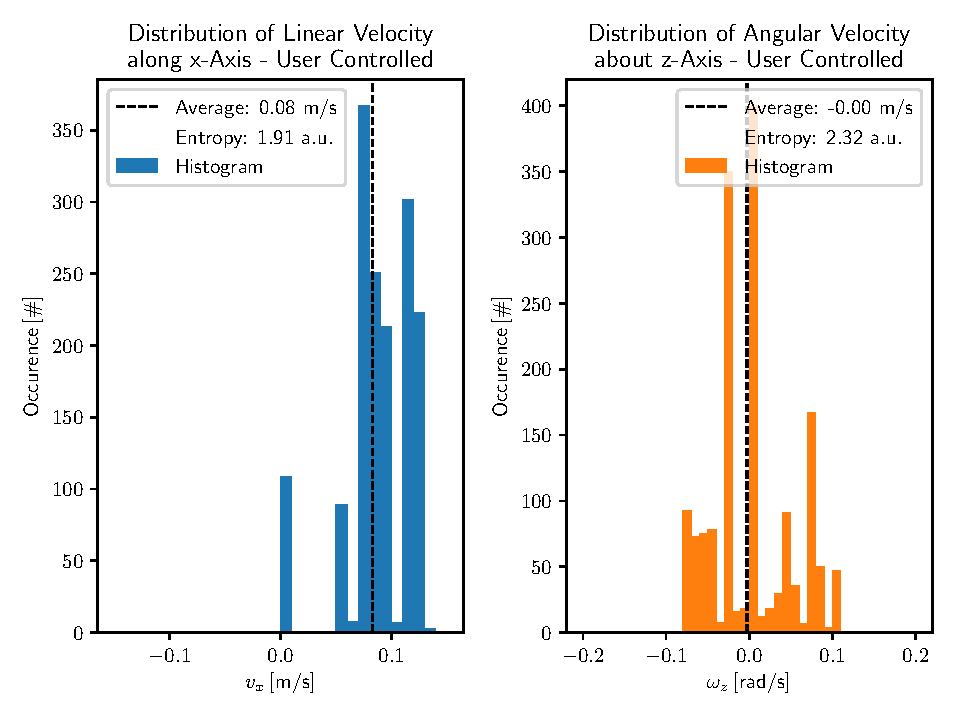
\includegraphics[scale=.35]{chapters/05_experiments/01_user_controlled_walking/02_test_environment/obstacle_walk_02_entropy.pdf}}
	\subcaptionbox{Environment Scanning - Dynamic Balance}%
	[.4\linewidth]{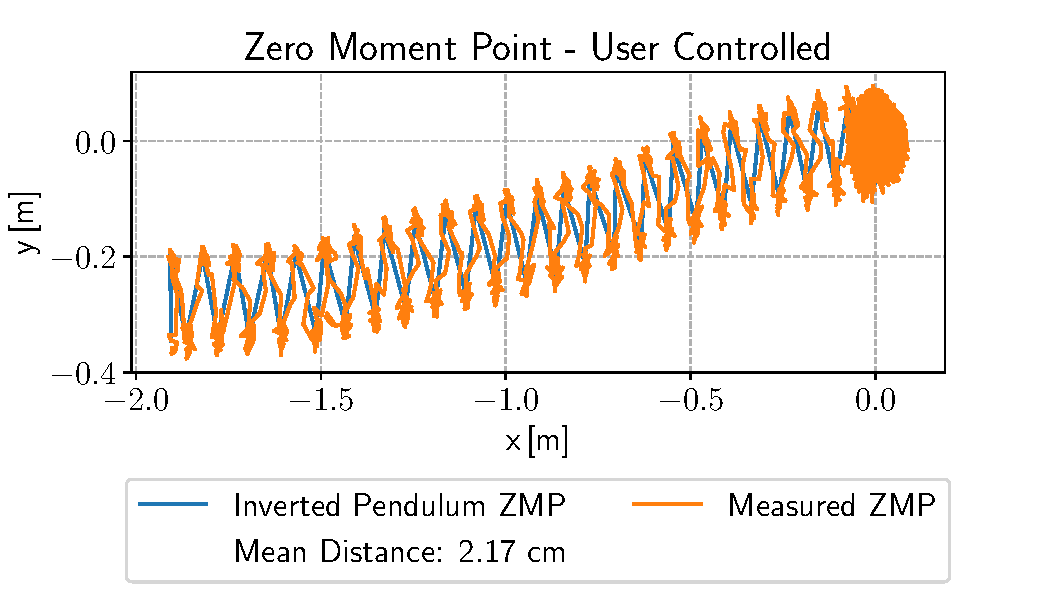
\includegraphics[scale=.35]{chapters/05_experiments/01_user_controlled_walking/02_test_environment/out_of_sight_walk_01_zmp.pdf}}
	\subcaptionbox{Environment Scanning - Behavior}%
	[.4\linewidth]{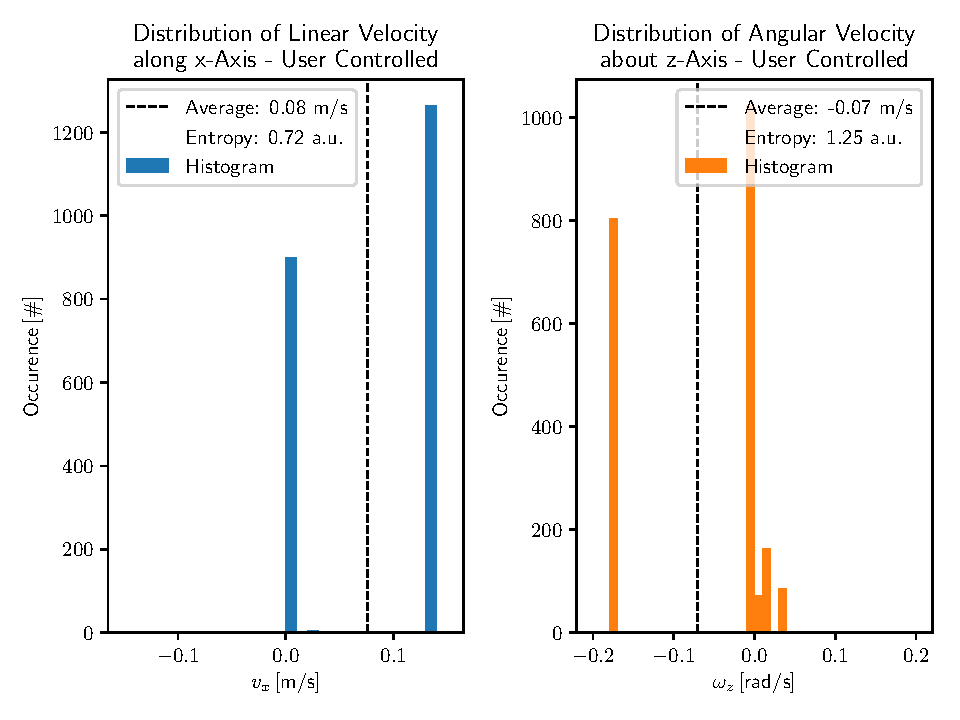
\includegraphics[scale=.35]{chapters/05_experiments/01_user_controlled_walking/02_test_environment/out_of_sight_walk_01_entropy.pdf}}
	\caption{}
	\label{fig::512_uc_basic}
\end{figure} 